\documentclass[onecolumn, crcready]{iosart2c}

\usepackage[english]{babel}
\usepackage[ampersand]{easylist}
\usepackage{graphicx} 
\usepackage{pdfpages}
\usepackage{fancyvrb}
\usepackage{pdflscape}
\usepackage{fancyhdr}
\usepackage{amssymb}
\usepackage{tabularx}
\usepackage{url}
\usepackage{listings}
\usepackage{lscape} 
\usepackage{multirow}
\usepackage{longtable}
\usepackage{tikz}
\usepackage{array}
\usepackage{booktabs}
\usepackage{rotating}


\setcounter{tocdepth}{3}
\graphicspath{ {figures/} }

\def\checkmark{\tikz\fill[scale=0.4](0,.35) -- (.25,0) -- (1,.7) -- (.25,.15) -- cycle;} 
\bibliographystyle{unsrt}


%\fancyhead[CO,CE]{---MidTerm Report--}
\fancyhead[RO, LE] {\thepage}
\renewcommand{\headrulewidth}{0.4pt}
\renewcommand{\footrulewidth}{0.4pt}

%%%%%%%%%%%%%%%%%%%%%%%%%%%%%%%
%%%  Beginning of document  %%%
%%%%%%%%%%%%%%%%%%%%%%%%%%%%%%%

\begin{document}

\begin{center}

\includegraphics[width=5cm]{EURECOM_logo_quadri}
\\[3cm]
\textbf{\Huge{MidTerm Report}}
\\[4cm]
\textbf{\LARGE{Self-Service Data Provisioning through Semantic Enrichment of Enterprise Data}}
\\[0.5cm]
\LARGE{Ahmad Assaf}
\\[0.5cm]
\small{EURECOM-Multimedia Communications}
\\
\large{Institut Mines-T\'{e}l\'{e}com}
\\
\large{December 15th, 2012}
\\[5cm]
\columnsep3cm
\begin{tabular}{p{8cm} p{8.5cm}}
\small{\textbf{Supervisors:}\newline
Rapha\"el Troncy \newline Aline Senart} 
&
\small{\textbf{\newline EURECOM\newline SAP}}
\end{tabular}
\end{center}

%%%%%%%%%%%%%%%%%%%%%%%%%%%%%%%%%
%%%  Chapter:Research Problems %%%
%%%%%%%%%%%%%%%%%%%%%%%%%%%%%%%%%

\section{Introduction}
Enterprises use a wide range of heterogeneous information systems in their business activities such as Enterprise Resource Planning (ERP), Customer Relationships Management (CRM) and Supply Chain Management (SCM) systems. An enterprise distributed IT landscape contains multiple systems using different technologies and data standards \cite{DBLP:conf/semweb/MihindukulasooriyaGG13}. In addition to this heterogeneity, the amount of information in enterprise databases and on-line data stores expands exponentially each year. Enterprise Big Data isn't big in volume only, but in the associated file formats also as the information is being stored often in unstructured and unknown formats.\\

Data Integration in large enterprises is a time and resource costly task. Various approaches have been introduced to solve this integration challenge. These approaches were primarily based on XML as the data representation syntax, Web Services to provide the data exchange protocols and Service Oriented Architecture (SOA) as a holistic approach for distributed systems architecture and communication \cite{frischmuth2103a}\cite{frischmuth2012linked}. However, it was found that these technologies are no sufficient to solve the integration problems in large enterprises. Recently, ontology-based data integration approaches have been suggested where ontologies are used to describe the data, queries and mappings between them \cite{Wache01ontology-basedintegration}. A slightly different approach is the use of the Linked Data paradigm \cite{bizer_linked_2009} for integrating enterprise data. Enterprises like Google and Microsoft are not only using the Linked Data integration paradigm for their information systems, but are also aiming at building enterprise knowledge bases ( like the Google Freebase\footnote{http://freebase.com}) that will act as a crystallization point for their structured data.\\

Linked Open Data (LOD) movement has gained lots of momentum in the last years. From 12 datasets cataloged in 2007, the Linked Open Data has grown to almost 300 datasets containing almost 32 billion triples \cite{bizer2011}. Data is being published by both public and private sectors and covers a diverse set of domains from life sciences to military. This success lies in the cooperation between data publishers and consumers. Users are empowered to find, share and combine information in their applications easily. 

Despite the legal issues surrounding Linked Data licenses \cite{nomoneyLOD}, it is still considered a gold mine for organizations who are trying to leverage external data sources in order to produce more informed business decisions \cite{Boyd2011}. In \cite{mckinseyreport} the authors see the potential economic effect unfolding in education, transportation, consumer products, electricity, oil and gas, health care and consumer finance. They estimate the potential annual value enabled by Open Data in these domains to reach 3 trillion US Dollars. 

Data becomes more useful when it is open, widely available and in shareable formats, and when advanced computing and analysis can yield from it. The quality and amount of structured knowledge available make it now feasible for companies to mine this huge amount of public data and integrate it in their next-generation enterprise information management systems. Analyzing this new type of data within the context of existing enterprise data should bring them new or more accurate business insights and allow better recognition of sales and market opportunities \cite{bigData}. 


%%%%%%%%%%%%%%%%%%%%%%%%%%%%%%
%%% section contributions %%%%
%%%%%%%%%%%%%%%%%%%%%%%%%%%%%%

\section{Challenges}
Business Intelligence has always been about creating new insight for business by converting data into meaning that can be shared between people to drive change in the organization. One key aspect of creating meaning is driving a common shared understanding of information also known as Semantics.

Classic BI and even the newer Agile Visualization tools focus much of their selling features on attractive and unique visualizations, but it still remains a truth that preparing data for those visualizations is the far more challenging task in most BI projects large and small. Self Service data provisioning aims at tackling this problem by providing datasets discovery, acquisition and integration techniques intuitively to the end user.

In this thesis, we aim at creating a framework that will leverage Semantic Web technologies in order to enrich enterprise data in general and Business Intelligence data in particular in order to facilitate self-serviced data provisioning. In this thesis, we investigate the following research challenges:

\begin{itemize}
\item The enterprise heterogeneous data sources raise tremendous challenges. They have inherently different file formats, access protocols or query languages. They possess their own data model with different ways of representing and storing the data. Data across these sources may be noisy (e.g. duplicate or inconsistent), uncertain or be semantically similar yet different \cite{OntologyBasedSemantic}. Integration and provision of a unified view for these heterogeneous and complex data structures therefore require powerful tools to map and organize the data.
\item Attaching metadata and Semantic information to instances can be tricky. An entity is usually not associated with a single generic type in the knowledge base, but rather with a set of specific types which can be relevant or not given the context. The challenging task is Finding the most relevant entity type within a given context.
\item Even though popular datasets like DBPedia\footnote{http://dbpedia.org} and Freebase are well known and widely used, there are other hidden useful datasets not being used. Indeed these datasets may be useful for specialized domains, however without proper registry of topics, it is difficult for users to find them \cite{AutomaticDomainIdentification}.
\item Linked Data consists of structured information supported by models, ontologies and vocabularies and contains query endpoints and links. This makes data quality assurance a challenge. Despite the fact that Linked Open Data quality is a trending and highly demanded topic, very few efforts are currently trying to standardize, track and formalize frameworks to issue scores or certificates that will help data consumers in their integration tasks.
\item Social Networks are not just gathering Internet users into groups of common interests, they are also helping people follow breaking news, contribute to online debates or learn from others. They are transforming Web usage in terms of users' initial entry point, search, browsing and purchasing behavior. Integrating information from these Social Networks can be tricky due to the vast amount of data available which makes hard to spot what is relevant in a timely manner.
\end{itemize}

\section{Proposal}


In order to enable self serviced data provisioning, we envisage building an indexing service (see Figure 1) that will be able to provide detailed data profiles for internal and external data sources. As a first step, we plan to build a data crawler that will be able to perform the following dataset discovery tasks on internal repositories and external Linked Data hubs:
 \begin{itemize}
 \item {\bf Data Acquisition}: Be able to sample data from the various datasets.
 \item {\bf Data Preparation}: This will include data profiling and validation, de-duplicating and enhancing relevant data sets with metadata. Profiling is used to examine data to understand its content, structure and data quality dependencies. The types of profiling tasks include:
 \begin{itemize}
 \item Examining column data and getting statistical information such as min, max, average, median, null percentage, value distribution, pattern distribution.
 \item Dependency tasks: Finds the values in one or more dependent columns that rely on values in a primary column
 \item Redundancy tasks: Determine the degree of overlapping data values or duplication between two sets of columns
 \item Uniqueness tasks: Returns the count and percentage of rows that contain non-unique data, for the set of column(s) selected.
 \item Content type: Content type profiling provides suggested meaning based on the entities data in the columns.
 \end{itemize}
 \item {\bf Dataset Classification}: Classify and organize datasets based on the input from the previous tasks.
\end{itemize}

Linked Open Data datasets are described using either the Vocabulary of Interlinked Datasets (VOID) \cite{Cyganiak:11:DLD} or the Data Catalog Vocabulary (DCAT) \cite{Maali:13:DCV}. With these standards, discovery and usage of linked datasets can be performed both effectively and efficiently. In our framework, we plan to use DCAT as the common standard for homogenizing description metadata of datasets indexed by our crawler. This choice came from the fact that the Open Data Support\footnote{http://opendatasupport.eu} is promoting the DCAT-AP (and consequently DCAT) as the standard for describing datasets and catalogs in Europe.

In addition to that, an important aspect that we have to take into consideration while describing a dataset is its quality. For that, an objective Linked Data quality assessment framework should be created in order to issue quality profiles that extend the DCAT vocabulary. The framework helps on one hand data owners to rate the quality of their dataset and get some hints on possible improvements, and on the other hand data consumers to choose their data sources from a ranked set. 

While Linked Data is a rich source of information, sometimes live information streamed from the Social Networks is needed. In addition to the Linked Data crawler, we will need to crawl Social Networks in order to aggregate semantically related information and connect it with the right resources. 

\begin{figure}[ht!]
  \centering
    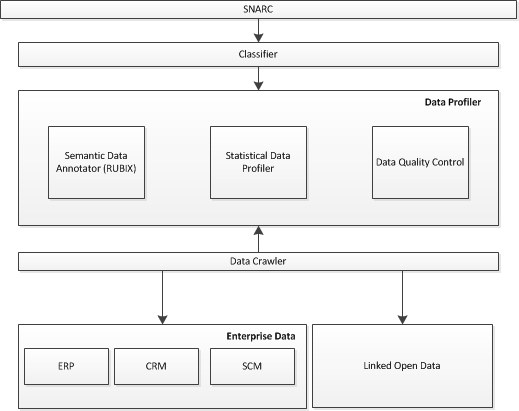
\includegraphics[scale=0.8]{overall-architecture.png} 
  \caption{Overall Architecture}
\end{figure}

\subsection{Contributions on Data Enrichment}
Regarding this aspect of our research, we have achieved the following tasks:
 \begin{itemize}
 \item Building RUBIX which is a framework enabling mash-up of potentially noisy enterprise and external data.
 \item RUBIX improves instance and schema matching by adding Semantic metadata to data at the instance level.
 \item RUBIX improves data integration techniques by enabling clean representation of the data regardless of the languages used, existence of abbreviations, synonyms and typos. 
 \item We presented RUBIX at the First International Workshop on Open Data \cite{Assaf:2012:RFI:2422604.2422607}\cite{DBLP:journals/corr/abs-1205-2691}.
\end{itemize}

\subsection{Contributions on Linked Data Quality}
Concerning our contributions on Linked Data quality assessment, we have achieved the following tasks:
\begin{itemize}
\item We identified five principle classes to describe the quality of a particular linked dataset. For each class, we list the principles that are involved at all stages of the data management process.
\item We have presented our Data quality principles at the Sixth IEEE International Conference on Semantic Computing \cite{assaf2012}.
\item We have surveyed the landscape of Linked Data quality assessment frameworks.
\item We have surveyed the landscape of Linked Data quality assessment tools.
\item We have refined the five principles in \cite{assaf2012} towards a more objective framework.
\item We have evaluated the surveyed tools with regards to the suggested framework.
\end{itemize}

\subsection{Contributions on Semantic Social Data Aggregation}
Concerning our contributions on Semantic Social data aggregation, we have achieved the following tasks:
\begin{itemize}
\item Build a Social crawler that queries several Social endpoints and aggregates news based on a set of defined keywords.
\item Build a common Semantic model to represent Web documents.
\item Building a Semantic Social News Aggregating service (SNARC) \cite{DBLP:conf/esws/AssafST13} that aggregates relevant Social news with regards to a Web document.
\item SNARC has won the first place at the AI Mashup Challenge\footnote{http://aimashup.org/aimashup13} at ESWC13.
\end{itemize}

%%%%%%%%%%%%%%%%%%%%%%%%%%%%%%%%%%%%
%%% Improving Data Integration with Linked Data %%%
%%%%%%%%%%%%%%%%%%%%%%%%%%%%%%%%%%%%

\section{Semantic Enrichment of Data}

Tagging and attaching metadata is often seen as additional work for data publishers with few paybacks. Moreover, different data creators use different terminologies which means that the same object maybe be represented using different metadata descriptions \cite{Furnas87thevocabulary}. Presenting and enterprise taxonomies requires a considerable amount of time and effort, at least in the initial creation steps \cite{frischmuth2012linked}.\\

RUBIX is our approach to bootstrap the process of attaching meta information to data objects. We leverage DBpedia and Freebase as knowledge bases for our annotation process. In RUBIX we assign a vector of Semantic types for every object at the instance level. For example, Orange will be represented by a vector of rich types that contain \texttt{(Organization, Organism Classification, Place ...)}. Currently, we rely on Freebase API to identify these rich types, but we have already started the effort to build an entity type ranking tool inspired by \cite{TRank}. 

\subsection{RUBIX to Enhance Schema Matching}

In the past, some work has tried to improve existing data schema \cite{DBLP:journals/debu/MillerA03} but literature mainly covers automatic or semi-automatic labeling of anonymous data sets through Web extraction. Examples include \cite{cas04} that automatically labels news articles with a tree structure analysis or \cite{wang2003extraction} that defines heuristics based on distance and alignment of a data value and its label. These approaches are however restricting label candidates to Web content from which the data was extracted. \cite{DBLP:conf/otm/SilvaBCS07} goes a step further by launching speculative queries to standard Web search engines to enlarge the set of potential candidate labels. More recently, \cite{Limaye:2010:ASW:1920841.1921005} applies machine learning techniques to respectively annotate table rows as entities, columns as their types and pairs of columns as relationships, referring to the YAGO ontology. The work presented aims however at leveraging such annotations to assist semantic search queries construction and not at improving schema matching. 
With the emergence of the Semantic Web, new work in the area has tried to exploit Linked Data repositories. The authors of \cite{Syed2010Tables} present techniques to automatically infer a semantic model on tabular data by getting top candidates from Wikitology \cite{conf/aaaiss/FininSMMP09} and classifying them with the Google page ranking algorithm. Since the authors' goal is to export the resulting table data as Linked Data and not to improve schema matching, some columns can be labeled incorrectly, and acronyms and languages are not well handled \cite{Syed2010Tables}. In the Helix project \cite{conf/www/HassanzadehDFKSW11}, a tagging mechanism is used to add semantic information on tabular data. A sample of instances values for each column is taken and a set of tags with scores are gathered from online sources such as Freebase. Tags are then correlated to infer annotations for the column. The mechanism is quite similar to ours but the resulting tags for the column are independent of the existing column name and sampling might not always provide a representative population of the instance values.\\

In RUBIX we have implemented several matching algorithms (Cosine Similarity, Pearson Product-Moment Correlation Coefficient (PPMCC) and Spearman's Rank Correlation Coefficient) in order to calculate similarity between data based on their rich types population. Our preliminary evaluation shows that for datasets where mappings were relevant yet not proposed, our framework provides higher quality matching results. Additionally, the number of matches discovered is increased when Linked Data is used in most datasets. 

\subsection{Dataset Annotation and Domain Identification}

The increasing diversity of the datasets makes it difficult to annotate them with a fixed number of pre-defined tags. Moreover, manually entered tags are subjective and may not capture the essence and breadth of the dataset \cite{AutomaticDomainIdentification}. RUBIX can be used to Annotate datasets with meta information based on examining the data instances themselves. In addition to that, we can enhance our approach by applying techniques similar to \cite{AutomaticDomainIdentification} in order to identify topical domains with fine-grained classification.


%%%%%%%%%%%%%%%%%%%%%%%%%%%%%%%%%%%%
%%% An Objective Assessment Framework for Linked Data Quality %%%
%%%%%%%%%%%%%%%%%%%%%%%%%%%%%%%%%%%%

\section{An Objective Assessment Framework for Linked Data Quality}

We are entering an era where open is the new default. Governments, universities, organizations and even individuals are publicly publishing huge amounts of open data.  This openness should be accompanied with a certain level of trust or guarantees about the quality of data.  To our knowledge, only one certificate is available to data publishers to assess the quality level of their datasets, the ODI certificate\footnote {https://certificates.theodi.org/}.\\

This certificate provides a description of the published data quality in plain English. It aspires to act as a mark of approval that helps publishers understand how to publish good open data and users how to use it. It gives publishers the ability to provide assurance and support on their data while encouraging further improvements through an ascending scale.

ODI comes as an online and free questionnaire for data publishers focusing on certain characteristics about their data. The questions are classified into the following categories: general information (about dataset, publisher and type of release), legal information (e.g., rights to publish), licensing, privacy (e.g., whether individuals can be identified), practical information (e.g., how to reach the data), quality, reliability, technical information (e.g., format and type of data) and social information (e.g., contacts, communities, etc.). Based on the information provided  by the data  publisher,  a certificate  is created  with one of four different ratings.\\

Although ODI is a great initiative, the issued certificates are “self-certified“. ODI does not verify or review submissions but retains the right to revoke a certificate at any time. The dynamicity of Linked Data  makes it also very difficult to update the certificates manually, especially when these changes are frequent and affect multiple categories. There is clearly a need for automatic certification which can be supplemented with some manual input for categories that cannot be processed by machines.\\


The emerging critical need for large, distributed, heterogeneous, and complex structured datasets identified the necessity to establish industry cooperation between vendors of RDF and Graph database technologies in developing, endorsing, and publishing reliable and insightful benchmark results. The Linked Data Benchmark Council (LDBC)\footnote{http://ldbc.eu/} aims to bridge the gap between the industry and the new trending stack of semantic technologies and their vendors. \\ LDBC more specifically aims at developing new benchmarks that will lead to significant progress in scalability, storage, indexing and query optimization techniques to become the de facto standard for publishing performance results. LDBC is promising initiative, but it is still work in progress with the final report expected on the first quarter of 2015.\\

In addition to the initiatives mentioned above, there exists a number of data quality frameworks and tools that are either standalone or implemented as modules in data integration tools. \\

LODGRefine\footnote{http://code.zemanta.com/sparkica/} is the Open Refine\footnote{http://openrefine.org/} of Linked Data. It does not act as a quality assessment tool, but it is powerful in cleaning and refining raw instance data. LODGRefine can help detect duplicates, empty values, spot inconsistencies, extract Named Entities, discover patterns and more. LODGRefine helps in improving the quality of the dataset by improving the quality of the data at the instance level.\\


PROLOD \cite{Bohm2010} is also not a quality assessment tool. It is a Linked Data profiling tool that provides clustering and labeling capabilities, schema discovery and statistics about data types and patterns. The statistics are about properties distribution, link-to-literal ratio, number of entities and RDF triples, average properties per entity and average error. PROLOD had been tested with DBpedia but the authors plan to improve its scalability to larger datasets.\\


Sieve \cite{Mendes2012} is framework for expressing quality assessment and fusion methods. It is implemented as a component of the Linked Data Integration Framework (LDIF)\footnote{http://ldif.wbsg.de/}. Sieve leverages the LDIF provenance metadata as quality indicators to produce quality assessment scores. However, despite its nice features, it is only targeted to perform data fusion based on user-configurable conflict resolution tasks. Moreover, since Sieve main input is provenance metadata, it is only limited to domains that can provide such metadata associated with their data.\\


Quality Assessment of Data Sources (Flemming's Data Quality Assessment Tool)\footnote{http://linkeddata.informatik.hu-berlin.de/LDSrcAss/datenquelle.php} calculates data quality scores based on manual user input. The user should assign weights to the predefined quality metrics and answer a series of questions regarding the dataset. These include, for example, the use of obsolete classes and properties by defining the number of described entities that are assigned disjoint classes, the usage of stable URIs and whether the publisher provides a mailing list for the dataset. The main disadvantage for using this tool is the manual intervention which requires deep knowledge in the dataset examined. Moreover, the tool lacks support for several quality concerns like completeness or consistency.\\


SWIQA \cite{Furber2011a} is composed of three layers: data acquisition, query and ontology layers. It uses query templates based on the SPARQL Inferencing Notation (SPIN)\footnote{http://spinrdf.org/} to express quality requirements. The queries are built to compute weighted and unweighted quality scores. At the end of the assessment, it uses vocabulary elements to annotate important values of properties and classes, assigning inferred quality scores to ontology elements and classifying the identified data quality problems.\\

Despite all the recent efforts in providing frameworks and tools for data quality in Linked Open Data, there is still no framework for the objective assessment of such quality taking into account all aspects of Linked Open Data.

In our previous work \cite{assaf2012} we have identified 24 different Linked Data quality attributes. We have refined these attributes into a condensed framework of 13 objective attributes. Since these attributes are rather abstract, we should rely on quality indicators that reflect data quality \cite{flemming2010}. In this paper, we transform the quality indicators presented as a set of questions in \cite{assaf2012} into more concrete quality indicator metrics. We extend them with the the objective quality indicators listed in the systematic review done in \cite{Framework2012}.\\

Table(1) lists the refined attributes along with their quality indicators. These attributes are:

\subsection{Objective Linked Data Quality Classification}
 \subsubsection{Completeness}

Data completeness can be judged in the presence of a task where the ideal set of attributes and objects are known. An entity is considered to be complete if it contains all the attributes needed for a given task, has complete language coverage \cite{Mader2012} and has documentation properties \cite{w3c_skos_rec}\cite{Mader2012}.\\ A dataset is considered to be complete if it contains all the necessary objects for a given task \cite{Mendes2012}, contains supporting structured metadata \cite{Hogan2010}, contains links for external data providers, supports providing data in multiple serializations \cite{Framework2012}, includes the correct MIME-type for the content \cite{Hogan2010}, contains appropriate volume of data for a particular task \cite{Framework2012}, has different queryable endpoints to access the data (i.e. SPARQL endpoint, RDF Dump, REST API, etc.) \cite{Framework2012}, has been checked against syntactic errors \cite{Hogan2010}, uses datasets description vocabularies like DCAT\footnote{http://www.w3.org/TR/vocab-dcat/} or VOID\footnote{http://www.w3.org/TR/void/} and if the publishers provide descriptions about the size (using void:statItem, void:numberOfTriples or void:numberOfDocuments) and categorization (using dcterms:subject) of the dataset.\\ Links are considered to be complete if all the in-bound and out-bound links are dereferenceable \cite{Hogan2010}\cite{Mader2012}\cite{Gueret2012} and have the linkage information represented in the metadata \cite{Hogan2010}.\\ Models are considered to be complete if they have a complete set of values \cite{Mader2012} and do not contain disconnected graph clusters \cite{Mader2012}. Disconnected graphs are the result of incomplete data acquisition or accidental deletion of terms that leads to deprecated terms. In addition to that, models are considered to be complete if they do not contain omitted top concepts or unidirectional related concepts \cite{Hogan2010} and if there exists some metadata about the kind and number of used vocabularies \cite{Framework2012}.

\subsubsection{Availability}

A dataset is considered to be available if the publishers provide an RDF dump that can be downloaded by users \cite{flemming2010}\cite{Hogan2010} and if its queryable endpoints respond to direct queries.

\subsubsection{Correctness}

Data correctness is related to the validity of its entities. An entity is considered to be correct if there are no missing or empty labels \cite{Acosta2013}\cite{Mader2012}, no incorrect data type for typed literals \cite{Hogan2010}\cite{Acosta2013}, no omitted or invalid languages tags \cite{Suominen:2012:IQS:2413941.2413985}\cite{Mader2012} and does not contain ``orphan terms'' (orphan terms are terms without any associative or hierarchical relationships \cite{journals/ires/Living10}).\\ Links are considered to be correct if they actually show related content to the subject of the RDF triple \cite{Suominen:2012:IQS:2413941.2413985}\cite{Acosta2013} and are syntactically correct. \\ Models are considered to be correct if the top concepts are marked and do not have broader concepts (for example having incoming hasTopConcept or outgoing topConceptOf relationships) \cite{Mader2012}.

\subsubsection{Conciseness}

Extensional conciseness measures the number of unique objects in relation to the overall number of objects representation in the dataset. Intensional conciseness measures the number of unique attributes of a dataset in relation to the overall number of attributes in a target schema \cite{ Bleiholder:2009}. \\ An entity is considered to be concise if it has intensional conciseness (it does not contain redundant attributes, which means that there is no equivalent attributes with different names) \cite{Mendes2012} and uses short URIs \cite{Framework2012} that follow the HTTP URI scheme \cite{Hogan:2012:ESL:2263498.2264570}\cite{Suominen2013}.\\ A dataset is considered to be concise if it has extensional conciseness (it does not contain redundant objects, which means that there is no equivalent objects with different identifiers) \cite{Mendes2012}.

\subsubsection{Consistency}

An entity is considered to be consistent if it does not contain overlapping labels such as two concepts have the same preferred lexical label in a given language when they belong to the same schema \cite{skosprimer}\cite{Mader2012}. Moreover, an entity is considered to be consistent if it does not contain disjoint labels \cite{Mader2012}, extra white spaces in labels \cite{Suominen:2012:IQS:2413941.2413985} and does not contain inconsistent preferred labels per language tag and no more than one value of skos:prefLabel without a language tag \cite{Mader2012}\cite{Suominen:2012:IQS:2413941.2413985}.\\ A dataset is considered to be consistent if it is free of conflicting information. This can be measured by considering properties with cardinality 1 that contain more than one distinct value \cite{Mendes2012}.\\ Models are considered to be consistent if they do not include atypical use of collections, containers and reification \cite{Hogan2010}, overlapping usage of owl:sameAs and owl:differentFrom \cite{Hogan2010}, overlapping usage of owl:AllDifferent and owl:distinctMembers \cite{Hogan2010}, asserted members of owl:Nothing and membership violation for disjoint classes \cite{Hogan2010}.

\subsubsection{Coherence}

Coherence is the ability to interpret data as expected by the publisher or vocabulary maintainer \cite{Hogan2010}. It is mainly associated with the modeling quality.\\ 

\noindent
A model is considered to be coherent when it does not contain:\\
\begin{easylist}[itemize]
\ListProperties( Hang=true, Progressive=3ex, Style*= - )
& Usage of undefined classes and properties \cite{Hogan2010}. Many errors that are due to spelling or syntactic mistakes are resolvable through minor fixes via ontology checkers tools. However, for new terms, \cite{Hogan2010} suggests to have them defined in a separate namespace in order to allow reuse \cite{ Mader2012}.
& Usage of blank nodes as they affect merging data from different sources \cite{Hogan:2012:ESL:2263498.2264570}.
& Misplaced or deprecated classes or properties \cite{Hogan2010}.
& Misuse of the owl:DataTypeProperty or owl:ObjectProperty \cite{Hogan2010}.
& Relations and mappings clashes \cite{Suominen:2012:IQS:2413941.2413985}.
& Invalid inverse-functional values \cite{Hogan2010}.
& Cyclic hierarchical relations \cite{conf/jcdl/Soergel05}\cite{Suominen:2012:IQS:2413941.2413985}\cite{Mader2012}.
& Incomplete literals with datatype range \cite{Hogan2010}.
& Solely transitive related concepts \cite{Mader2012}.
& Redefinitions of existing vocabularies \cite{Hogan2010}.
& Valueless associative relations \cite{Mader2012}.
\end{easylist}

\subsubsection{Efficiency}

Dataset efficiency is calculated by measuring how fast it can be identified \cite{Toupikov2009}. A dataset is considered to be efficient if it satisfies the following performance metrics:\\
\begin{easylist}[itemize]
\ListProperties( Hang=false, Progressive=3ex, Style*= - )
& No usage of slash-URIs where large amounts of data is provided \cite{Framework2012}.
& Acceptable delay between the request and its response \cite{citeulike:2925559}.
& Low Latency HTTP requests (average answer time of one second) \cite{Framework2012}.
& Scalable such that the time to answer an amount of ten requests divided by ten is not longer than the time it takes to answer one request \cite{Framework2012}.
\end{easylist}

\subsubsection{Freshness}

Freshness is a measure for the recency of data. The basic assumption is that old information is more likely to be outdated and unreliable \cite{Flouris2012}. Entity freshness can be identified if it contains timestamps that can keep track of its modifications.

\subsubsection{Accuracy}

Accuracy describes the proximity of data value representations of an object related to their real world states \cite{Furber2011a}. A dataset is considered to be accurate when it does not contain outliers and attributes that do not contain useful values for data entries \cite{Framework2012}.

\subsubsection{Provenance}

Entity level provenance can be calculated by constructing decision networks informed by provenance graphs \cite{Gamble2011}. The accuracy of computing trust between two entities \cite{Framework2012} can be computed by calculating an aggregate trust value based on the combination of the propagation and aggregation algorithms on weighted mechanism \cite{j.websem208}. Provenance can be achieved at the dataset level by including metadata that describes its authoritative information (title, content and URI), ensuring the reliability and trustworthiness of the publisher \cite{Flouris2012}, verifying if the dataset uses a provenance vocabulary like PROV \cite{w3c-prov-o} and uses digital signatures \cite{Framework2012}. \\ Models provenance can be achieved by ensuring the trustworthiness of RDF statements \cite{Hartig09usingweb}. 

\subsubsection{Security}

Security is a quality attribute that is measured on the dataset level. It is identified if the publishers use login credentials, SSL or SSH to provide access to their dataset, or if they only grant access to specific users \cite{Framework2012}.

\subsubsection{Licensing}

Licensing is a quality attribute that is measured on the dataset level. It includes the availability of machine readable license information \cite{Hogan:2012:ESL:2263498.2264570}, human readable license information in the documentation of the dataset or its source \cite{Hogan:2012:ESL:2263498.2264570} and the indication of permissions, copyrights and attributions specified by the author \cite{Framework2012}.

\subsubsection{Comprehensibility}

Comprehensibility is identified if the publisher indicates at least one exemplary URI and SPARQL query, regular expression pattern that matches the URIs of a dataset \cite{Framework2012} and if he provides a list of used vocabularies and an active mailing list or message board for the dataset \cite{flemming2010}. 

\begin{landscape}
\begin{center}
{\footnotesize
\begin{longtable}[h]{|c|c|c|c|}
\caption[Objective Assessment Framework for Linked Data Quality]{Objective Assessment Framework for Linked Data Quality} \label{DQM} \\

\hline \multicolumn{1}{|c|}{\textbf{Quality Attribute}} & \multicolumn{1}{c|}{\textbf{Quality Category}} & \multicolumn{1}{c|}{\textbf{ID}} & \multicolumn{1}{c|}{\textbf{Quality Indicator}} \\ \hline
\endfirsthead

\multicolumn{4}{c}%
{{\bfseries \tablename\ \thetable{} Objective Assessment Framework for Linked Data Quality}} \\
\hline \multicolumn{1}{|c|}{\textbf{Quality Attribute}} &
\multicolumn{1}{c|}{\textbf{Quality Category}} & \textbf{ID} &
\multicolumn{1}{c|}{\textbf{Quality Indicator}} \\ \hline 
\endhead

\multicolumn{4}{|r|}{{Continued on next page}} \\ \hline
\endfoot


\endlastfoot
 
\multirow{19}{*}{Completeness} & \multirow{3}{*}{Entity Level} & QI.1 & Covers of all the attributes needed for a given task \cite{Mendes2012}\tabularnewline
\cline{3-4} 
 &  & QI.2 & Has complete language coverage \cite{Mader2012}\tabularnewline
\cline{3-4} 
 &  & QI.3 & Existence of documentation properties  \cite{w3c_skos_rec}\cite{Mader2012}\tabularnewline
\cline{2-4} 
 & \multirow{9}{*}{Dataset Level} & QI.4 & Existence of all the necessary objects for a given task \cite{Mendes2012}\tabularnewline
\cline{3-4} 
 &  & QI.5 & Existence of supporting structured metadata  \cite{Hogan2010}\tabularnewline
\cline{3-4} 
 &  & QI.6 & Supports multiple serializations \cite{Framework2012}\tabularnewline
\cline{3-4} 
 &  & QI.7 & Includes the correct MIME-type for the content  \cite{Hogan2010}\tabularnewline
\cline{3-4} 
 &  & QI.8 & Contains appropriate volume of data for a particular task \cite{Framework2012}\tabularnewline
\cline{3-4} 
 &  & QI.9 & Has different queryable endpoints to access the data \cite{Framework2012}\tabularnewline
\cline{3-4} 
 &  & QI.10 & Checked against syntactic errors \cite{Hogan2010}\tabularnewline
\cline{3-4} 
 &  & QI.11 & Usage of datasets description vocabularies \tabularnewline
\cline{3-4} 
 &  & QI.12 & Existence of descriptions about its size and categorization \tabularnewline
\cline{2-4} 
 & \multirow{2}{*}{Links Level} & QI.13 & Existence of complete dereferenceable in-bound and out-bound links \cite{Hogan2010}\cite{Mader2012}\cite{Gueret2012}\tabularnewline
\cline{3-4} 
 &  & QI.14 & Existence of supporting linkage metadata  \cite{Hogan2010}\tabularnewline
\cline{2-4} 
 & \multirow{5}{*}{Model Level} & QI.15 & Covers the complete set of values \cite{Mader2012}\tabularnewline
\cline{3-4} 
 &  & QI.16 & Absence of disconnected graph clusters \cite{Mader2012}\tabularnewline
\cline{3-4} 
 &  & QI.17 & Absence of omitted top concept \cite{Hogan2010}\tabularnewline
\cline{3-4} 
 &  & QI.18 & Absence of unidirectional related concepts \cite{Hogan2010}\tabularnewline
\cline{3-4} 
 &  & QI.19 & Existence of supporting metadata about the kind and number of used vocabularies \cite{Framework2012}\tabularnewline
\hline 
\hline 
\multirow{2}{*}{Availability} & \multirow{2}{*}{Dataset Level} & QI.20 & Existence of an RDF dump that can be downloaded by users \cite{flemming2010}\cite{Hogan2010}\tabularnewline
\cline{3-4} 
 &  & QI.21 & Existence of queryable endpoints that respond to direct queries\tabularnewline
\hline 
\hline 
\multirow{8}{*}{Correctness} & \multirow{4}{*}{Entity Level} & QI.22 & Absence of missing or empty labels \cite{Acosta2013}\cite{Mader2012}\tabularnewline
\cline{3-4} 
 &  & QI.23 & Absence of incorrect data type for typed literals \cite{Hogan2010}\cite{Acosta2013} \tabularnewline
\cline{3-4} 
 &  & QI.24 & Absence of omitted or invalid languages tags \cite{Suominen:2012:IQS:2413941.2413985}\cite{Mader2012}\tabularnewline
\cline{3-4} 
 &  & QI.25 & Absence of terms without any associative or hierarchical relationships \cite{journals/ires/Living10}\tabularnewline
\cline{2-4} 
 & \multirow{2}{*}{Links Level} & QI.26 & Existence of content related to the subject of the RDF triple \cite{Suominen:2012:IQS:2413941.2413985}\cite{Acosta2013}\tabularnewline
\cline{3-4} 
 &  & QI.27 & Absence of syntactic errors  \cite{Suominen2013}\tabularnewline
\cline{2-4} 
 & \multirow{2}{*}{Model Level} & QI.28 & Contains marked top concepts \cite{Mader2012}\tabularnewline
\cline{3-4} 
 &  & QI.29 & Absence of broader concepts for top concepts \cite{Mader2012}\tabularnewline
\hline 
\hline 
\multirow{4}{*}{Conciseness} & \multirow{2}{*}{Entity Level} & QI.30 & Absence of redundant attributes \cite{Mendes2012}\tabularnewline
\cline{3-4} 
 &  & QI.31 & Existence of short URIs \cite{Framework2012}\tabularnewline
\cline{2-4} 
 & \multirow{2}{*}{Dataset Level} & QI.32 & Absence of redundant objects \cite{Mendes2012}\tabularnewline
\cline{3-4} 
 &  & QI.33 & Follows the HTTP URI scheme \cite{Hogan:2012:ESL:2263498.2264570}\cite{Suominen2013}\tabularnewline
\hline  
\hline 
\multirow{3}{*}{Security} & \multirow{3}{*}{Dataset Level} & QI.34 & Uses login credentials to restrict access \cite{Framework2012}\tabularnewline
\cline{3-4} 
 &  & QI.35 & Uses SSL or SSH to provide access to their dataset \cite{Framework2012}\tabularnewline
\cline{3-4} 
 &  & QI.36 & Grants access to specific users \cite{Framework2012}\tabularnewline
\hline 
\hline 
\multirow{1}{*}{Freshness} & \multirow{1}{*}{Entity Level} & QI.37 & Existence of timestamps that can keep track of its modifications  \cite{Flouris2012}\tabularnewline
\hline 
\hline 
\multirow{3}{*}{Licensing} & \multirow{3}{*}{Dataset Level} & QI.38 & Existence of machine readable license information \cite{Hogan:2012:ESL:2263498.2264570}\tabularnewline
\cline{3-4} 
 &  & QI.39 & Existence of human readable license information  \cite{Hogan:2012:ESL:2263498.2264570}\tabularnewline
\cline{3-4} 
 &  & QI.40 & Specifies permissions, copyrights and attributions  \cite{Framework2012}\tabularnewline
\hline 
\hline 
\multirow{5}{*}{Comprehensibility} & \multirow{5}{*}{Dataset Level} & QI.41 & Existence of at least one exemplary URI \cite{Framework2012}\tabularnewline
\cline{3-4} 
 &  & QI.42 & Existence of at least one exemplary SPARQL query \cite{Framework2012}\tabularnewline
\cline{3-4} 
 &  & QI.43 & Existence of regular expression pattern that matches the URIs of a dataset \cite{Framework2012}\tabularnewline
\cline{3-4} 
 &  & QI.44 & Existence of a list of used vocabularies \tabularnewline
\cline{3-4} 
 &  & QI.45 & Existence of a mailing list or message board \cite{flemming2010}\tabularnewline
\hline 
\multirow{11}{*}{Consistency} & \multirow{5}{*}{Entity Level} & QI.46 & Existence of consistent preferred labels per language tag \cite{skosprimer}\cite{Mader2012}\tabularnewline
\cline{3-4} 
 &  & QI.47 & Absence of overlapping labels\tabularnewline
\cline{3-4} 
 &  & QI.48 & Absence of disjoint labels \cite{Mader2012}\tabularnewline
\cline{3-4} 
 &  & QI.49 & Absence of extra white spaces in labels \cite{Suominen:2012:IQS:2413941.2413985}\tabularnewline
\cline{3-4} 
 &  & QI.50 & Existence of only one value of skos:prefLabel without a language tag  \cite{Mader2012}\cite{Suominen:2012:IQS:2413941.2413985}\tabularnewline
\cline{2-4} 
 & \multirow{1}{*}{Dataset Level} & QI.51 & Absence of conflicting information \cite{Mendes2012}\tabularnewline
\cline{2-4} 
 & \multirow{5}{*}{Model Level} & QI.52 & Absence of atypical use of collections, containers and reification \cite{Hogan2010}\tabularnewline
\cline{3-4} 
 &  & QI.53 & Absence of overlapping usage of owl:sameAs and owl:differentFrom  \cite{Hogan2010}\tabularnewline
\cline{3-4} 
 &  & QI.54 & Absence of overlapping usage of owl:AllDifferent and owl:distinctMembers  \cite{Hogan2010}\tabularnewline
\cline{3-4} 
 &  & QI.55 & Absence of asserted members of owl:Nothing  \cite{Hogan2010}\tabularnewline
\cline{3-4} 
 &  & QI.56 & Absence of membership violations for disjoint classes  \cite{Hogan2010}\tabularnewline
\hline 
\hline 
\multirow{10}{*}{Coherence} & \multirow{10}{*}{Model Level} & QI.57 & Absence of misplaced or deprecated classes or properties  \cite{Hogan2010}\tabularnewline
\cline{3-4} 
 &  & QI.58 & Absence of misused owl:DataTypeProperty or owl:ObjectProperty  \cite{Hogan2010}\tabularnewline
\cline{3-4} 
 &  & QI.59 & Absence of relation and mappings clashes  \cite{Suominen:2012:IQS:2413941.2413985}\tabularnewline
\cline{3-4}
 &  & QI.60 & Absence or minimal usage of blank nodes \cite{Hogan:2012:ESL:2263498.2264570}\tabularnewline
\cline{3-4} 
 &  & QI.61 & Absence of invalid inverse-functional values \cite{Hogan2010}\tabularnewline
\cline{3-4} 
 &  & QI.62 & Absence of cyclic hierarchical relations \cite{conf/jcdl/Soergel05}\cite{Suominen:2012:IQS:2413941.2413985}\cite{Mader2012}\tabularnewline
\cline{3-4} 
 &  & QI.63 & Absence of undefined classes and properties usage \cite{Hogan2010}\tabularnewline
\cline{3-4} 
 &  & QI.64 & Absence of solely transitive related concepts \cite{Mader2012}\tabularnewline
\cline{3-4} 
 &  & QI.65 & Absence of redefinitions of existing vocabularies  \cite{Hogan2010}\tabularnewline
\cline{3-4} 
 &  & QI.66 & Absence of valueless associative relations  \cite{Mader2012}\tabularnewline
\cline{3-4} 
 &  & QI.67 & Absence of incomplete literals with datatype range \cite{Hogan2010}\tabularnewline
\hline 
\hline 
\multirow{4}{*}{Efficiency} & \multirow{4}{*}{Dataset Level} & QI.68 & Absence of slash-URIs \cite{Framework2012}\tabularnewline
\cline{3-4} 
 &  & QI.69 & Acceptable delay between the request and its response \cite{citeulike:2925559}\tabularnewline
\cline{3-4} 
 &  & QI.70 & Low Latency HTTP requests \cite{Framework2012}\tabularnewline
\cline{3-4} 
 &  & QI.71 & Ability to scale \cite{Framework2012}\tabularnewline
\hline 
\hline 
\multirow{2}{*}{Accuracy} & \multirow{2}{*}{Dataset Level} & QI.72 & Absence of outliers \cite{Framework2012}\tabularnewline
\cline{3-4} 
 &  & QI.73 & Absence of attributes that do not contain useful values for data entries \cite{Framework2012}\tabularnewline
\hline
\hline
\multirow{6}{*}{Provenance} & \multirow{1}{*}{Entity Level} & QI.74 & Ability to construct decision networks informed by provenance graphs \cite{Gamble2011}\tabularnewline
\cline{2-4} 
 & \multirow{4}{*}{Dataset Level} & QI.75 & Existence of metadata that describes its authoritative information  \cite{Flouris2012}\tabularnewline
\cline{3-4} 
 &  & QI.76 & Reliability and Trustworthiness of the publisher \cite{Flouris2012}\tabularnewline
\cline{3-4} 
 &  & QI.77 & Usage of a provenance vocabulary\tabularnewline
\cline{3-4} 
 &  & QI.78 & Usage of digital signatures \cite{Framework2012}\tabularnewline
\cline{2-4} 
 & \multirow{1}{*}{Model Level} & QI.79 & Trustworthiness of RDF statements \cite{Hartig09usingweb}\tabularnewline
\hline
\end{longtable}
}
\end{center}
\end{landscape}

\subsection{Linked Data Quality Tools}
In this section, we present the results of our survey on the Linked Data quality tools that reflect the different aspects of LOD: modeling, ontologies and vocabularies, dataset and SPARQL end-points.\\


\subsubsection{Information Modeling Quality}
RDF is the standard to model information in the Semantic Web. Linked Data publishers can pick from a plethora of tools that can check their RDF files for quality problems\footnote{http://www.w3.org/2001/sw/wiki/SWValidators}. Syntactic RDF checkers are able to detect errors in RDF documents like the W3C RDF Validator\footnote{http://www.w3.org/RDF/Validator/}, RDF:about validator and Converter\footnote{http://rdfabout.com/demo/validator/} and The Validating RDF Parser (VRP)\footnote{http://139.91.183.30:9090/RDF/VRP/index.html}. The RDF Triple-Checker\footnote{http://graphite.ecs.soton.ac.uk/checker/} is an online tool that helps find typos and common errors in RDF data. Vapour\footnote{http://validator.linkeddata.org/vapour} \cite{Berrueta08cookinghttp} is a validation service to check whether semantic Web data is correctly published according to the current best practices\cite{tim:linkedata}.

\subsubsection {Ontologies and Vocabularies Quality}
Reusing existing ontologies is a common practice that Linked Data publishers are always trying to adopt. However, ontologies and vocabularies development is often a long error-prone process especially when many contributors are working consecutively or collaboratively \cite{Suominen2013}. This can introduce deficiencies such as redundant concepts or conflicting relationships \cite{harpring_introduction_2010}. Getting to choose the right ontology or vocabulary is vital to ensure modeling correctness and consistency.\\ qSKOS\footnote{https://github.com/cmader/qSKOS} \cite{Mader2012} scans SKOS vocabularies to provide reports on vocabulary resources and relations that are problematic. Skosify \cite{Suominen:2012:IQS:2413941.2413985} supports OWL and RDFS ontologies by converting them into well-structured SKOS vocabularies. Skosify includes automatic correction abilities for quality issues that have been observed by reviewing vocabularies on the Web. The OOPS! pitfall scanner \cite{oops} evaluates OWL ontologies against a rules catalog and provides the user with a set of guidelines to solve them. PoolParty checker\footnote{http://www.poolparty.biz/} highlights quality issues in OWL, RDFS and SKOS ontologies and vocabularies, the latest version supports qSKOS to indicate the quality of controlled vocabularies on the Web. ASKOSI\footnote{http://www.w3.org/2001/sw/wiki/ASKOSI} retrieves vocabularies from different sources, stores and displays the usage frequency of the different concepts used by different applications. It promotes reusing existing information systems by providing better management and presentation tools.\\ Some errors in RDF will only appear after reasoning (incorrect inferences). In \cite{conf/owled/SirinSW08}\cite{conf/hicss/TaoDM09} the authors perform quality checking on OWL ontologies using integrity constraints involving the Unique Name Assumption (UNA) and the Closed World Assumption (CWA). Pellet\footnote{http://clarkparsia.com/pellet} provides reasoning services for OWL ontologies. It incorporates a number of heuristics to detect and repair quality issues among disjoint properties, negative property assertions and reflexive, irreflexive, symmetric, and anti-symmetric properties. Eyeball\footnote{http://jena.sourceforge.net/Eyeball/} provides quality inspection for RDF models (including OWL). It provides checks for a variety of problems including the usage of unknown predicates, classes, poorly formed namespaces, literal syntax validation, type consistency and other heuristics. RDF:Alerts\footnote{http://swse.deri.org/RDFAlerts/} provides validation for many issues highlighted in \cite{Hogan2010} like misplaced, undefined or deprecated classes or properties. 

\subsubsection {Dataset Quality}
Considering the large amount of available datasets in the Linked Open Data, users have a hard time trying to identify appropriate datasets that suit certain tasks. There are two approaches to rank datasets, a manual and an automatic approach. The manual approach depends on the wisdom of the crowd to highlight specific quality issues. The automatic approach has several implementations. The most adopted ones are based on link assessment. Provenance-based approaches and entity-based approaches are also used to compute not only dataset rankings, but also rankings on the entity level.\\

\noindent
{\bf Manual Ranking Tools}\\

There are several quality issues that can be difficult to spot and fix automatically. In \cite{Acosta2013} the authors highlight the fact that the RDFification process of some data can be more challenging than others, leading to errors in the Linked Data provisioning process that needs manual intervention. This can be more visible in datasets that have been semi-automatically translated to RDF from their primary source (the best example for this case is DBpedia \cite{bizer_dbpedia_2009}). The authors introduce a methodology to adjust crowdsourcing input from two types of audience: 1) Linked Data experts, researchers and enthusiasts through a contest to find and classify erroneous RDF triples and 2) Crowd-sourcing through the Amazon Mechanical Turk\footnote{https://www.mturk.com/}.\\ TripleCheckMate \cite{Kontokostas2013} is the tool used by the authors to run out their assessment. The tool allows users to select resources, identify and classify possible issues according to a pre-defined taxonomy of quality problems. It measures inter-rater agreements, meaning that the resources defined are checked multiple times. These features turn out to be extremely useful to analyze the performance of users and allow better identification of potential quality problems. TripleCheckMate is used to identify accuracy issues in the object extraction (completeness of the extraction value for object values and datatypes), relevancy of the extracted information, representational consistency and interlinking with other datasets.\\

\noindent
{\bf Automatic Ranking Tools}\\ \\
{\bf Links Based Approach}\\

The basic idea behind link assessment tools is to provide rankings for datasets based on the cardinality and types of the relationships with other datasets. Traditional link analysis has proven to be an effective way to measure the quality of Web documents search. Algorithms like PageRank \cite{Lawrence981} and HITS \cite{Kleinberg:1999} became successful based on the assumption that a certain Web document is considered to have higher importance or rank if it has more incoming links that other Web documents \cite{Brin:1998}\cite{Chakrabarti99miningthe}.\\ However, the basic assumption that links are equivalent does not suit the heterogeneous nature of links in the Linked Open Data. Thus, the previous approaches fall short to provide reliable rankings as the types of the links can have a direct impact on the ranking computation \cite{Toupikov2009}.\\ The first adaption of PageRank for Semantic Web resources was the Ontology Rank algorithm implemented in the Swoogle search engine \cite{Ding2004}. They use a rational random surfing model that takes into account the different types of links between discovered sets and compute rankings based on three levels of granularity: documents, terms and RDF graphs. ReConRank \cite{Hogan06reconrank:a} rankings are computed at query time based on two levels of granularity: resources and context graphs. DING \cite{Toupikov2009} adapted the PageRank to rank datasets based on their interconnections. DING can also automatically assign weights to different link types based on the nature of the predicate involved in the link.\\Broken links are a major threat to Linked Data. They occur when resources are removed, moved or updated. DSNotify\footnote{http://www.cibiv.at/~niko/dsnotify/}\cite{cs142} is a framework that informs data consumers about the various types of events that occur on data sources. Their approach is based on an indexing infrastructure that extracts feature vectors and stores them to an index. A monitoring module detects events on sources and write them to a central event log which pushes notifications to registered applications.\\

{\bf Provenance-based Approach}\\

Provenance-based assessment methods are an important step towards transparency of data quality in the Semantic Web. In \cite{Hartig09usingweb} the authors use a provenance model as an assessment method to evaluate the timeliness of Web data. Their model identifies types of ``provenance elements'' and the relationships between them. Provenance elements are classified into three types: actors, executions and artifacts. The assessment procedure is divided into three steps: 1) Creating provenance graph based on the defined model 2) Annotating the graph with impact values 3) Calculating the information quality score. In \cite{Flouris2012} the authors describe a set of provenance-based assessment metrics to support quality assessment and repair in Linked Open Data. They rely on both data and metadata and use indicators like the source reputation, freshness and plausibility. In \cite{Harth2009} the authors introduce the notion of naming authority which connects an identifier with the source to establish a connection to it's provenance. They construct a naming authority graph that acts as input to derive PageRank scores for the data sources.\\

{\bf Entity-based Approach}\\

Sindice \cite{Delbru2010} uses a set of techniques to rank Web data. They use a combination of query dependent and query independent rankings implemented in the Semantic Information Retrieval Engine (SIREn)\footnote{http://siren.sindice.com/} to produce a final entity rank. Their query dependent approach rates individual entities by aggregating the the score of the matching terms with a term frequency - inverse subject frequency (tf-isf) algorithm. Their query independent ranking is done using hierarchical links analysis algorithms \cite{Delbru2010a}. The combination of these two approaches is used to generate a global weighted rank based on the dataset, entities and links ranks. \\


\subsubsection{Queryable End-point Quality}
The availability of Linked Data is highly dependent on the performance qualities of its queryable end-points. The standard query language for Semantic Web resources is SPARQL, thus SPARQL endpoints are the main focus. In \cite{Buil-Aranda2013} the authors present their findings to measure the discoverability of SPARQL endpoints by analyzing how they are located and the metadata used to describe them. In addition to that, they also analyze endpoints interoperability by identifying features of SPARQL 1.0 and SPARQL 1.1 that are supported. The authors tackled the endpoints efficiency by testing the time taken to answer generic, content-agnostic SPARQL queries over HTTP. Finally, the authors measured endpoints reliability by monitoring the uptime of public SPARQL endpoints on a course of 27 months. The results for this work can be accessed online via the SPARQL Endpoints Status tool \footnote{http://labs.mondeca.com/sparqlEndpointsStatus/} and is queryable using their public SPARQL endpoint\footnote{http://labs.mondeca.com/sparqlEndpointsStatus/endpoint/endpoint.html}. \\

\subsection{Linked Data Quality Tools Evaluation}
In this section, we present the results for our evaluation of the various Linked Data tools mentioned with regards to the presented framework (Table 2). Due to space limitation, we have only shown the tools that can directly or indirectly assess one or more of the quality indicators listed in Table 1. Moreover, we have also grouped the Syntax Validation tools (W3C RDF Validator, RDF:about, VRP, The RDF Triple-Checker and Vapour) under one approach. We should highlight that the PoolParty tool includes qSKOS in its implementation, thus they are grouped in one tool which is the PoolParty.\\

\newcolumntype{P}[2]{%
  >{\begin{turn}{#1}\begin{minipage}{#2}\small\raggedright\hspace{0pt}}l%
  <{\end{minipage}\end{turn}}%
}

\begin{center}
{\footnotesize
\begin{longtable}[h]{|c|c|c|c|c|c|c|c|c|c|c|c|c|c|c|c|c|}
\caption[Linked Data quality tools]{Evaluation of Linked Data quality tools for each quality indicator} \label{DQMT} \\

\hline \multicolumn{1}{|c|}{\textbf{}} & \multicolumn{1}{P{90}{3.1cm}|}{PROLOD} & \multicolumn{1}{P{90}{3.1cm}|}{Sieve} & \multicolumn{1}{P{90}{3.1cm}|}{Flemming's Tool}& \multicolumn{1}{P{90}{3.1cm}|}{SWIQA} & \multicolumn{1}{P{90}{3.1cm}|}{Syntax Validators}& \multicolumn{1}{P{90}{3.1cm}|}{Skosify} & \multicolumn{1}{P{90}{3.1cm}|}{OOPS!} & \multicolumn{1}{P{90}{3.1cm}|}{PoolParty} & \multicolumn{1}{P{90}{3.1cm}|}{ASKOSI} & \multicolumn{1}{P{90}{3.1cm}|}{Pellet} & \multicolumn{1}{P{90}{3.1cm}|}{Eyeball} & \multicolumn{1}{P{90}{3.1cm}|}{RDF:Alerts} & \multicolumn{1}{P{90}{3.1cm}|}{TripleCheckmate} & \multicolumn{1}{P{90}{3.1cm}|}{DING} & \multicolumn{1}{P{90}{3.1cm}|}{DSNotify} & \multicolumn{1}{P{90}{3.1cm}|}{SPARQL Endpoints-Status}\\ \hline 
\endfirsthead

\multicolumn{17}{c}%
{{\bfseries \tablename\ \thetable{} Evaluation of Linked Data quality tools for each quality indicator}} \\
\hline \multicolumn{1}{|c|}{\textbf{}} & \multicolumn{1}{P{90}{3.1cm}|}{PROLOD} & \multicolumn{1}{P{90}{3.1cm}|}{Sieve} & \multicolumn{1}{P{90}{3.1cm}|}{Flemming's Tool}& \multicolumn{1}{P{90}{3.1cm}|}{SWIQA} & \multicolumn{1}{P{90}{3.1cm}|}{Syntax Validators}& \multicolumn{1}{P{90}{3.1cm}|}{Skosify} & \multicolumn{1}{P{90}{3.1cm}|}{OOPS!} & \multicolumn{1}{P{90}{3.1cm}|}{PoolParty} & \multicolumn{1}{P{90}{3.1cm}|}{ASKOSI} & \multicolumn{1}{P{90}{3.1cm}|}{Pellet} & \multicolumn{1}{P{90}{3.1cm}|}{Eyeball} & \multicolumn{1}{P{90}{3.1cm}|}{RDF:Alerts} & \multicolumn{1}{P{90}{3.1cm}|}{TripleCheckmate} & \multicolumn{1}{P{90}{3.1cm}|}{DING} & \multicolumn{1}{P{90}{3.1cm}|}{DSNotify} & \multicolumn{1}{P{90}{3.1cm}|}{SPARQL Endpoints-Status} \\ \hline 
\endhead

\hline \multicolumn{17}{|r|}{{Continued on next page}} \\ \hline
\endfoot

\hline
\endlastfoot


\hline 
QI.1 &  & \checkmark &  & \checkmark &  &  &  &  &  &  &  &  & \checkmark &  &  & \tabularnewline
\hline 
QI.2 &  &  & \checkmark &  &  &  &  & \checkmark & \checkmark &  &  &  &  &  &  & \tabularnewline
\hline 
QI.3 &  &  & \checkmark &  &  &  &  & \checkmark &  &  &  &  &  &  &  & \tabularnewline
\hline 
QI.4 &  & \checkmark &  & \checkmark &  &  &  &  &  &  &  &  & \checkmark &  &  & \tabularnewline
\hline 
QI.5 &  &  & \checkmark &  &  &  &  &  &  &  &  &  &  &  &  & \tabularnewline
\hline 
QI.6 &  &  & \checkmark &  &  &  &  &  &  &  &  &  &  & \checkmark &  & \tabularnewline
\hline 
QI.7 &  &  & \checkmark &  &  &  &  &  &  &  &  &  &  &  &  & \tabularnewline
\hline 
QI.8 & \checkmark &  & \checkmark &  &  &  &  &  &  &  &  &  &  &  &  & \tabularnewline
\hline 
QI.9 &  &  & \checkmark &  &  &  &  &  &  &  &  &  &  &  &  & \tabularnewline
\hline 
QI.10 &  &  & \checkmark & \checkmark & \checkmark &  &  &  &  &  &  & \checkmark &  &  &  & \tabularnewline
\hline 
QI.11 &  &  &  &  &  &  &  &  &  &  &  &  &  & \checkmark &  & \checkmark\tabularnewline
\hline 
QI.12 & \checkmark &  & \checkmark &  &  &  &  &  &  &  &  &  &  & \checkmark &  & \tabularnewline
\hline 
QI.13 & \checkmark &  & \checkmark & \checkmark &  &  &  & \checkmark &  &  &  & \checkmark &  &  & \checkmark & \tabularnewline
\hline 
QI.14 &  &  &  &  &  &  &  &  &  &  &  &  &  &  & \checkmark & \checkmark\tabularnewline
\hline 
QI.15 &  & \checkmark &  & \checkmark &  &  &  &  &  &  &  &  &  &  &  & \tabularnewline
\hline 
QI.16 &  &  &  &  &  &  &  & \checkmark &  &  &  &  &  &  &  & \tabularnewline
\hline 
QI.17 &  &  &  &  &  & \checkmark &  & \checkmark &  &  &  &  &  &  &  & \tabularnewline
\hline 
QI.18 &  &  &  &  &  & \checkmark &  & \checkmark &  &  &  &  &  &  &  & \tabularnewline
\hline 
QI.19 &  &  & \checkmark &  &  &  &  &  &  &  &  &  &  &  &  & \tabularnewline
\hline 
QI.20 &  &  & \checkmark &  &  &  &  &  &  &  &  &  &  &  &  & \tabularnewline
\hline 
QI.21 &  &  & \checkmark &  &  &  &  &  &  &  &  &  &  &  &  & \checkmark\tabularnewline
\hline 
QI.22 & \checkmark &  &  &  &  & \checkmark &  & \checkmark & \checkmark &  &  &  & \checkmark &  &  & \tabularnewline
\hline 
QI.23 &  &  &  &  &  &  & \checkmark &  &  & \checkmark & \checkmark & \checkmark & \checkmark &  &  & \tabularnewline
\hline 
QI.24 &  &  &  &  &  & \checkmark &  & \checkmark &  &  &  &  &  &  &  & \tabularnewline
\hline 
QI.25 &  &  &  &  &  &  &  & \checkmark & \checkmark &  &  &  &  &  &  & \tabularnewline
\hline 
QI.26 &  &  &  &  &  &  &  &  &  &  &  &  &  &  &  & \tabularnewline
\hline 
QI.27 &  & \checkmark &  &  &  &  &  &  &  &  & \checkmark & \checkmark &  &  & \checkmark & \tabularnewline
\hline 
QI.28 &  &  &  &  &  & \checkmark &  & \checkmark &  &  &  &  &  &  &  & \tabularnewline
\hline 
QI.29 &  &  &  &  &  &  & \checkmark & \checkmark & \checkmark &  & \checkmark &  &  &  &  & \tabularnewline
\hline 
QI.30 &  & \checkmark &  & \checkmark &  &  & \checkmark &  & \checkmark &  &  &  &  &  &  & \tabularnewline
\hline 
QI.31 &  &  &  &  &  &  &  &  &  &  &  &  &  &  &  & \tabularnewline
\hline 
QI.32 &  & \checkmark &  & \checkmark &  &  &  &  &  &  &  &  &  &  &  & \tabularnewline
\hline 
QI.33 &  &  &  &  &  &  &  & \checkmark &  &  &  & \checkmark &  &  &  & \tabularnewline
\hline 
QI.34 &  &  &  &  &  &  &  &  &  &  &  &  &  &  &  & \tabularnewline
\hline 
QI.35 &  &  &  &  &  &  &  &  &  &  &  &  &  &  &  & \tabularnewline
\hline 
QI.36 &  &  &  &  &  &  &  &  &  &  &  &  &  &  &  & \tabularnewline
\hline 
QI.37 &  & \checkmark &  & \checkmark &  &  &  &  &  &  &  &  &  &  &  & \tabularnewline
\hline 
QI.38 &  &  & \checkmark &  &  &  &  &  &  &  &  &  &  &  &  & \tabularnewline
\hline 
QI.39 &  &  & \checkmark &  &  &  &  &  &  &  &  &  &  &  &  & \tabularnewline
\hline 
QI.40 &  &  & \checkmark &  &  &  &  &  &  &  &  &  &  &  &  & \tabularnewline
\hline 
QI.41 &  &  & \checkmark &  &  &  &  &  &  &  &  &  &  &  &  & \tabularnewline
\hline 
QI.42 &  &  & \checkmark &  &  &  &  &  &  &  &  &  &  &  &  & \tabularnewline
\hline 
QI.43 &  &  & \checkmark &  &  &  &  &  &  &  &  &  &  &  &  & \tabularnewline
\hline 
QI.44 &  &  & \checkmark &  &  &  &  &  &  &  &  &  &  &  &  & \tabularnewline
\hline 
QI.45 &  &  & \checkmark &  &  &  &  &  &  &  &  &  &  &  &  & \tabularnewline
\hline 
QI.46 &  &  &  &  &  & \checkmark &  & \checkmark & \checkmark &  &  &  &  &  &  & \tabularnewline
\hline 
QI.47 &  &  &  &  &  &  & \checkmark & \checkmark &  &  & \checkmark &  &  &  &  & \tabularnewline
\hline 
QI.48 &  &  &  &  &  & \checkmark & \checkmark & \checkmark &  &  & \checkmark &  &  &  &  & \tabularnewline
\hline 
QI.49 &  &  &  &  &  & \checkmark &  &  &  &  & \checkmark &  &  &  &  & \tabularnewline
\hline 
QI.50 &  &  &  &  &  &  &  &  & \checkmark &  &  &  &  &  &  & \tabularnewline
\hline 
QI.51 &  & \checkmark &  &  &  &  &  &  &  & \checkmark & \checkmark &  & \checkmark &  &  & \tabularnewline
\hline 
QI.52 &  &  &  &  &  &  &  &  &  &  & \checkmark &  &  &  &  & \tabularnewline
\hline 
QI.53 &  &  &  &  &  &  & \checkmark &  &  & \checkmark &  &  &  &  &  & \tabularnewline
\hline 
QI.54 &  &  &  &  &  &  &  &  &  & \checkmark &  &  &  &  &  & \tabularnewline
\hline 
QI.55 &  &  &  &  &  &  &  &  &  & \checkmark &  &  &  &  &  & \tabularnewline
\hline 
QI.56 &  &  & \checkmark &  &  & \checkmark & \checkmark & \checkmark &  & \checkmark & \checkmark & \checkmark &  &  &  & \tabularnewline
\hline 
QI.57 &  &  &  &  &  &  & \checkmark & \checkmark &  &  & \checkmark & \checkmark &  &  &  & \tabularnewline
\hline 
QI.58 &  &  &  &  &  &  & \checkmark &  &  & \checkmark & \checkmark &  &  &  &  & \tabularnewline
\hline 
QI.59 &  &  &  &  &  &  &  & \checkmark &  &  &  &  &  &  &  & \tabularnewline
\hline 
QI.60 &  &  &  &  &  &  &  &  &  &  &  &  &  &  &  & \tabularnewline
\hline 
QI.61 &  &  & \checkmark &  &  &  & \checkmark &  &  & \checkmark &  & \checkmark &  &  &  & \tabularnewline
\hline 
QI.62 &  &  &  &  &  & \checkmark & \checkmark & \checkmark & \checkmark &  &  &  &  &  &  & \tabularnewline
\hline 
QI.63 &  &  & \checkmark &  &  &  & \checkmark & \checkmark &  & \checkmark & \checkmark &  &  &  &  & \tabularnewline
\hline 
QI.64 &  &  &  &  &  & \checkmark & \checkmark & \checkmark &  &  &  &  &  &  &  & \tabularnewline
\hline 
QI.65 &  &  & \checkmark &  &  &  & \checkmark &  &  & \checkmark & \checkmark &  &  &  &  & \tabularnewline
\hline 
QI.66 &  &  &  &  &  &  &  & \checkmark &  &  &  &  &  &  &  & \tabularnewline
\hline 
QI.67 &  &  &  &  &  &  & \checkmark & \checkmark &  & \checkmark & \checkmark & \checkmark &  &  &  & \tabularnewline
\hline 
QI.68 &  &  & \checkmark &  &  &  &  &  &  &  &  &  &  &  &  & \tabularnewline
\hline 
QI.69 &  &  &  &  &  &  &  &  &  &  &  &  &  &  &  & \checkmark\tabularnewline
\hline 
QI.70 &  &  & \checkmark &  &  &  &  &  &  &  &  &  &  &  &  & \checkmark\tabularnewline
\hline 
QI.71 &  &  &  &  &  &  &  &  &  &  &  &  &  &  &  & \checkmark\tabularnewline
\hline 
QI.72 &  &  &  &  &  &  &  &  &  &  &  &  & \checkmark &  &  & \tabularnewline
\hline 
QI.73 &  &  &  &  &  &  &  &  &  &  &  &  & \checkmark &  &  & \tabularnewline
\hline 
QI.74 &  &  &  &  &  &  &  &  &  &  &  &  &  &  &  & \tabularnewline
\hline 
QI.75 &  &  & \checkmark &  &  &  &  &  &  &  &  &  &  &  &  & \tabularnewline
\hline 
QI.76 &  &  &  &  &  &  &  &  &  &  &  &  &  &  &  & \tabularnewline
\hline 
QI.77 &  &  & \checkmark &  &  &  &  &  &  &  &  &  &  &  &  & \tabularnewline
\hline 
QI.78 &  &  & \checkmark &  &  &  &  &  &  &  &  &  &  &  &  & \tabularnewline
\hline 
QI.79 &  &  &  &  &  &  &  &  &  &  &  &  &  &  &  & \tabularnewline
\end{longtable}
}
\end{center}

As a result, we have identified the need for a complete quality framework that can assess all the quality indicators. Most of the tools were designed with limited coverage to certain aspects, for example, ontology and vocabulary checkers focus mainly on the coherence, completeness and correctness at the modeling level. Flemming's tool covers several attributes like the completeness, correctness, conciseness, security, licensing and comprehensibility, but it falls short in measuring the consistency, coherence, efficiency and provenance.\\

We have also noticed the lack of tools to measure certain quality indicators like the dataset's security. Moreover, to our knowledge, there are no tools that can measure all the provenance quality indicators (except for Flemming's tool that is able to check for the use of digital signatures) although the literature covers several approaches to achieve that \cite{Hartig09usingweb}\cite{Flouris2012}\cite{Harth2009}.

%%%%%%%%%%%%%%%%%%%%%%%%%%%%%%%%%%%%
%%%  Semantic Social News Aggregation %%%
%%%%%%%%%%%%%%%%%%%%%%%%%%%%%%%%%%%%
\section{Semantic Social News Aggregation}

The Internet has created a paradigm shift in how we consume and disseminate information. Data nowadays is spread over heterogeneous silos of archived and live data. People willingly share data on social media by posting news, views, presentations, pictures and videos. SNARC is a service that uses semantic web technology and combines services available on the web to aggregate social news. SNARC brings live and archived information to the user that is directly related to his active page. The key advantage is an instantaneous access to complementary information without the need to dig for it. Information appears when it is relevant enabling the user to focus on what is really important.

Crawling data from these heterogeneous platforms implies the studying of related API specifications which differ in terms of use, privacy policy and described methods. Harvesting content spread over multiple platforms is a challenging task that has to ensure an easy and flexible way for integrating several social Web APIs. Tools such as API Blender \cite{journals/corr/abs-1301-2086} or Media Finder \cite{conf/chi/KangS03} provide such interface with the aim to save developers' efforts for learning each API specification. However, for in SNARC we needed services that are not available in the mentioned services. As a result, we have implemented our own Social crawler for Twitter\footnote{http://www.twitter.com}, Google+\footnote{http://plus.google.com}, YouTube\footnote{http://www.youtube.com}, Vimeo\footnote{http://www.vimeo.com}, Slideshare\footnote{http://www.slideshare.com}, Stack Exchange \footnote{http://stackexchange.com/}and the Web.

\subsection{Underlying Mechanism}
The back-end of SNARC consists of three major components: a document handler that creates a \"Semantic Model\" that represents any web resource, a query layer that is responsible for disseminating queries to the supported social services and a data parser which processes the search results, wraps them in a common social model and generates the desired output.

\subsubsection{Document Handler}
The main idea behind SNARC is to provide a uniform model for web entities, whether they are blog entries, multimedia objects or micro-posts. To do so, SNARC creates a \"Semantic Model\" containing all the annotations and meta-data needed to query and reconcile social results. 
\begin{figure}[ht!]
  \centering
    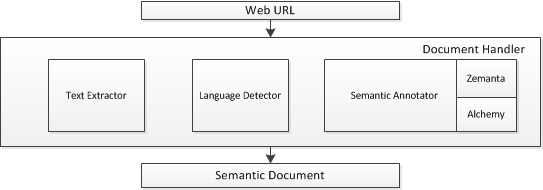
\includegraphics[scale=0.8]{architecture-part1.png} 
  \caption{SNARC's Document Handler}
\end{figure}

The Semantic Model is created by the Document Handler (see Figure 1) which receives a web page URL and performs these three main steps:
\begin{enumerate}
\item {\bf Text Extraction:} Fetch the webpage that corresponds to the received URL and extract the textual content using a set of heuristics. These latter identify the main content of the page by stripping unwanted HTML tags and rank the different sections based on their semantics, class names and order. In the beginning we have used Alchemy API\footnote{http://www.alchemyapi.com} to perform text extraction; but we have chosen to implement a simpler method ourselves which saved us an extra API call. 
\item {\bf Language Detection:} Detect the web page language using the Language Detection service of Alchemy API. This is necessary to match the desired language with compatible services like Twitter, YouTube, etc.
\item {\bf Semantic Annotation:} Annotating the extracted text is the most important step in this process. We use Zemanta Suggest\footnote{http://developer.zemanta.com/docs/suggest/} and Alchemy API in order to extract: 
\begin{itemize}
\item {\bf Tags:} These are the finest-grained queryable \"keywords\" that we use to retrieve the social results. From our experiments, combining tags results in better findings than using entities or concepts. However, we plan to evaluate the combination of keywords, entities and concepts in order to find the top-queryable terms that will retrieve the most relevant results on different abstraction levels.
\\Tags retrieved from these services are ranked by confidence values calculated by their internal algorithms, these values are normalized for each service. According to our experiments we have found that Alchemy's Keywords Extraction API returns a large set of closely related keywords (i.e. Android, Android Phone, Android Tablet, ...). To construct a good query we therefore need to provide a certain level of abstraction.We perform a cleaning process on those keywords by applying the Levenshtein distance to rule out closely related keywords by disregarding those with lower confidences. We perform a similar process on the result of the union between the keywords returned by Alchemy and Zemanta to ensure a sparse keywords set.
\item {\bf Semantic Entities:} Entities provide a higher abstraction level of the document. They are used to reconcile the social results in order to maintain relevancy with the document. Similar to the keywords extraction services, the entities retrieved are ranked and contain outbound links to the matched entity on dbpedia, Wikipedia, Freebase, etc. A union is made between the results from Alchemy and Zemanta to ensure a wider coverage of entities. When a match is found, we merge the links from the two sources to ensure that we include all the resources that can be used to augment extra information about that entity in the document. 
\item {\bf Categories:} These are high-level taxonomies that can generally describe the document's content. A taxonomy is used to narrow down our query scope when targeting services like YouTube. In our Semantic Document model we define two possible category sets, one retrieved from Alchemy's Text Categorization API\footnote{http://www.alchemyapi.com/api/categ/categs.html} and the other retrieved from Zemanta Suggest API that follows the DMOZ categorization scheme\footnote{http://www.dmoz.org/desc/Top}.
\end{itemize}
\end{enumerate}
At the end of this process, we will have constructed the needed elements (keywords, entities and high level categories) wrapped in our Semantic Model to be passed to the query generator. For example, a summary of the Semantic Model for a web page titled \"Turkey protests: Erdogan in \'final\' warning\footnote{http://www.bbc.co.uk/news/world-europe-22889060}\"  looks like: 
\begin{enumerate}
\item {\bf Categories:} Culture\_Politics, Regional and Society
\item {\bf Keywords:} Taksim Square, Protesters, Gezi Park, Mr Erdogan, Istanbul ...
\item {\bf Entities:} Gezi Park, Recep Tayyip Erdogan, Taksim Square, Justice and Development Party (Turkey), Police of Turkey ...
\end{enumerate}

\subsubsection{Query Layer}
In this component, the calls to the social services are made. SNARC uses the extracted keywords from the Semantic Document in order to construct the queries and disseminate them to the appropriate services. Figure 2 shows the different steps in order to retrieve a set of social results.
\begin{figure}[ht!]
  \centering
    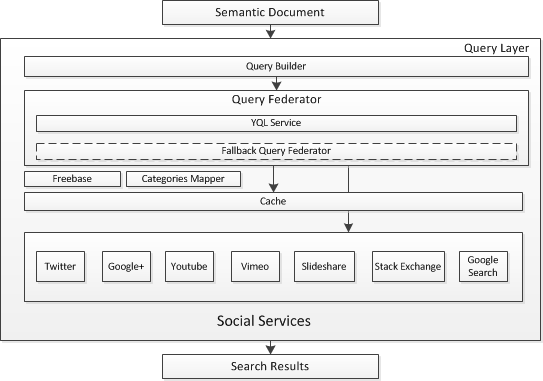
\includegraphics[scale=0.75]{architecture-part2.png}
  \caption{SNARC's Query Layer}
\end{figure}

\begin{enumerate}
\item {\bf Query Builder:} Responsible for identifying targeted services and building tailored queries for each service. For example, if the processed document is categorized as a computer or technology related one, Stackoverflow service will be targeted with the queries constructed. However, other categories will correspond to different services from the Stack Exchange websites\footnote{http://stackexchange.com/sites}.
\item {\bf Query Federator:} Responsible for federating the queries identified in the previous step to the corresponding services. To enhance performance, we tried to reduce the number of external calls. Yahoo Query Language (YQL)\footnote{http://developer.yahoo.com/yql/} helped us in minimizing the number of calls and batching them into a single one. It is an expressive SQL-like language that lets you query, filter, and join data across Web services. However, we have found that we cannot fully rely on YQL due to their API calls limit and the restriction on the query execution time that is set to 30 seconds. To overcome this, we have implemented a fallback mechanism that federates the queries to the selected social services and groups the result to be passed afterwards to the parser. \\
To further optimize the number of calls, we have decided to take the top two ranked keywords. We do not apply logical operator (AND/OR) in our queries; instead, we perform one-to-one mapping between each keyword and query. Indeed, we have found that gathering keywords even if semantically related might bring up noise in the results. However, as mentioned earlier, a part of the future work will be investigating the best method to construct the most relevant queryable entity using different logical operators.
\item {\bf Caching:}The main setback in the query layer was the variable limited number of calls we can make to external APIs. To overcome this, we have implemented a simple cache mechanism that saves the results on disk up to an hour. There are several cache levels; the first is a URL level one where the results of the parsed queries are cached. For example, if a user visited a certain article on the CNN webpage the results might take up to 15 seconds to appear, whereas a second user visiting the same article minutes afterwards will have the cached results in few seconds. The second level is keyword and service specific. This can be very helpful as users generally browse articles of related topics or interests (semantic concepts), so for each user we can end up with the same high level concepts being requested frequently. An important thing to note is that the caching is done on the server side and is disk-based.
\end{enumerate}
The social services queried can be grouped as follows:
\begin{enumerate}
\item {\bf Multimedia Services:} They include Slideshare, Vimeo and YouTube. Slideshare and YouTube allow the results to be fetched in a specific language that was detected in the previous step. In addition to that, YouTube search services are called twice; the first call is done to the YouTube V2 API\footnote{https://developers.google.com/youtube/2.0/} where we specify in addition to the keywords a high level category to be targeted. To do so, we have manually created a category mapping file that maps the high-levels categories of Alchemy’s API and DMOZ to those provided by YouTube. The second call is done to YouTube V3 API\footnote{https://developers.google.com/youtube/v3/}. The new feature provided by Google in this version is the ability to search using a semantic concept that corresponds to a Freebase concept ID; it proves to retrieve better results that the normal search. Freebase concept calls are cached for longer periods as they are less prone to changes. 
\item {\bf Micro-posts Services:} They include Twitter, Google+ and Stackoverflow. Language filtering is done where applicable. 
\item {\bf General Search:} This includes similar results found via Google search or those retrieved from the Zemanta API call. They are general articles or blog posts related to the current active page.
\end{enumerate}
\subsubsection{Data Parser}
This is the last step where the results and unified and wrapped in a single social model. Figure 3 shows the different steps needed to produce the final parsed results that will be pushed back to the front-end.
\begin{figure}[ht!]
  \centering
    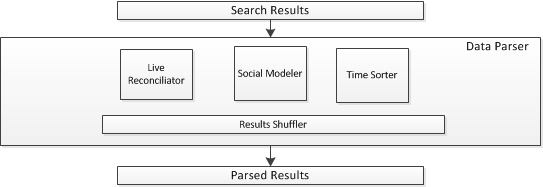
\includegraphics[scale=0.8]{architecture-part3.png} 
  \caption{SNARC's Data Parser}
\end{figure}

\begin{enumerate}
\item {\bf Live Reconciliator:} Social (or folksonomic) tagging has become a trending method to describe, search and discover content on the web. Folksonomies empower users by giving them total freedom in choosing their categories and keywords that they think describe best the content. This contrasts with taxonomies that over-impose hierarchical categorization of content \cite{Zanardi2008}. However, in services like Twitter and Google+, tagging has been abused in a way that increased noise in the stream of results. To overcome this problem, we align the incoming stream of posts with the set of semantic concepts or keywords that describe the document. There are several approaches and tools like \cite{Cantador2011,Diaz-Aviles2012,Preotiuc-Pietro2012,Zanardi2008} that aim at solving this problem. In SNARC we rely on two levels of reconciliation: one uses the high-level taxonomy (categories); and the other uses the vector of entities defined in the Semantic Document. For example, if SNARC wants to reconcile a blog post result retrieved from a general search, it constructs a Semantic Document Model for that result and applies the Cosine Similarity on the vector of ranked entities for each Semantic Model. Currently, we only reconcile against blog posts as it is very straightforward to construct a Semantic Document Model for them. However, an integral part of the future work will be the integration of SNARC's model to micro-posts and video search services.

\item {\bf Social Modeler:} Every social network has its own underlying data model. To overcome this problem, we need to present the social results in a common wrapper. To do so, we have created an optimized universal social model that contains all the necessary data to model social information and can be reused in other projects. The model contains service related attributes like the service name and type, general post information like the author's name, profile link, image and geo-location information and post-specific information like the title, thumbnail, embed code, main content and link. 
\item {\bf Time Sorter and Results Shuffler:} To better display the results on the front-end, we unify the time representation and sort the results based on it. Afterwards we pick the top N results and shuffle them to generate a random order.
\end{enumerate}


%%%%%%%%%%%%%%%%%%%%%%%%%%%%%%%%%%%%
%%%  Conclusions and Future Work %%%
%%%%%%%%%%%%%%%%%%%%%%%%%%%%%%%%%%%%

\section{Conclusions and Future work}

We have presented in this document our main contributions in some issues around Enriching Enterprise Data Towards Self-Service Data Provisioning. We have first focused on the aspect of data profiling through RUBIX. We plan to extend RUBIX to be able to work with DBpedia leveraging the planned entity type ranking module. We also plan to include data mining techniques to profile numerical data and provide statistical insights about data distribution. 

Regarding the Linked Data quality module, we plan to develop a comprehensive objective Linked Data quality evaluation tool. The tool will be able to automatically measure the various quality indicators listed in this paper, introduce a scoring function with different weights for the various quality attributes and issue a quality certificate.

Regarding the Social integration, we would like to test SNARC on business web application, check if our annotations can be used to successfully query and attach relevant social snippets to the data.

We also plan to build our Linked Data crawler that will be responsible for the data acquisition phase which is the entry point for the work done so far. We also plan to investigate possible extensions to the current data description vocabularies to allow more comprehensive datasets categorization. 


\nocite{*}
\bibliographystyle{amsplain}
\bibliography{biblio}

\end{document}